This chapter surveys the freelance-platform landscape, derives the actors and use cases relevant to FreelanceChain, and specifies functional and non-functional requirements.

\section{Status Survey}
\label{section:2.1}

\subsection{Existing Platforms}

The dominant centralized platforms are Upwork and Fiverr, supplemented by Toptal and Freelancer.com. Upwork's published fee policy applies a tiered rate (a sliding 5--20\% based on client--freelancer earnings history)~\cite{upworkfees2024}, while disputes are handled through the platform's internal Trust \& Safety process and escrowed funds reside in commercial bank accounts. Fiverr operates a flat 20\% commission on a gig-based model~\cite{fiverrfees2024}, which is reported to accommodate complex multi-deliverable engagements poorly. Ethlance, the earliest decentralized alternative, advertises zero platform fees and full on-chain transparency~\cite{ethlance2018}, but its public repositories show limited maintenance activity since 2018 and its reliance on Ethereum mainnet fees discourages small-value engagements. Colony and Braintrust target team-oriented task management and talent-network governance respectively~\cite{colony2020whitepaper,braintrust2021whitepaper}, rather than direct freelance project matching. Based on these public sources, no surveyed decentralized system simultaneously addresses escrow, reputation, identity, governance, and AI-assisted evaluation in a single program. Table~\ref{table:platform_comparison} summarizes the comparison; each row is annotated with the source from which the corresponding value was taken.

\begin{table}[H]
\centering
\caption{Comparison of major freelance platforms. Sources: Upwork~\cite{upworkfees2024,upwork2023}; Fiverr~\cite{fiverrfees2024,fiverr2023}; Toptal~\cite{toptal2024policy}; Ethlance~\cite{ethlance2018}; Colony~\cite{colony2020whitepaper}; Braintrust~\cite{braintrust2021whitepaper}.}
\label{table:platform_comparison}
\small
\begin{tabular}{|l|c|c|c|c|c|c|}
\hline
\textbf{Feature} & \textbf{Upwork} & \textbf{Fiverr} & \textbf{Toptal} & \textbf{Ethlance} & \textbf{Braintrust} & \textbf{FreelanceChain} \\ \hline
Service fee & 5--20\% & 20\% & client side & 0\% & 10\% (client) & 0\% (Devnet) \\ \hline
Escrow custody & Platform & Platform & Platform & Contract & Contract & Contract \\ \hline
Dispute resolution & Platform & Platform & Platform & None & DAO (limited) & On-chain \\ \hline
Reputation portability & No & No & No & Limited & Limited & Yes (SBT) \\ \hline
Identity verification & Centralized & Centralized & Manual & None & KYC partner & Browser biometric \\ \hline
Governance & Operator & Operator & Operator & None & Token-based DAO & DAO (prototype) \\ \hline
Milestone escrow & Yes & Partial & Yes & No & Yes & Yes \\ \hline
Active maintenance & Active & Active & Active & Limited (post-2018) & Active & Active (prototype) \\ \hline
\end{tabular}
\end{table}

\noindent Some cells in Table~\ref{table:platform_comparison} are intentionally coarse: feature lists evolve, and several platforms publish only partial documentation. The references should be consulted for the exact terms in force at the time of writing.

\subsection{User Survey: Methodology and Findings}
\label{subsection:2.1.2}

\textbf{Survey design.} A small-scale informal questionnaire was conducted between September and November 2025 to elicit candidate pain points for requirements analysis. The survey is exploratory rather than statistically representative; its primary purpose is to corroborate the structural deficiencies identified from secondary sources (Section~\ref{section:1.1}) and to inform the use-case prioritization of this prototype. The full questionnaire is reproduced in Appendix~\ref{appendix:survey} for reference.

\textbf{Participants.} Thirty respondents participated voluntarily: twenty self-identified as freelancers (predominantly software developers, UI/UX designers, and content writers) and ten as clients who had hired freelancers within the preceding twelve months. Respondents were recruited via convenience sampling through Vietnamese freelance-developer Telegram and Facebook groups; the sample is therefore biased toward Vietnam-based technical professionals and is not representative of the global freelance population. No identifying personal data was collected, and participation was anonymous.

\textbf{Instrument.} The questionnaire comprised twelve closed-form items (Likert-scale ratings of perceived pain points, prior experience with Web3 wallets, willingness to use a decentralized alternative) and four open-ended items. The full item list is given in Appendix~\ref{appendix:survey}.

\textbf{Findings.} Within this small and self-selected sample, the most frequently reported pain points, in descending order, were: platform fees reducing net income (85\% of freelancer respondents); perceived unfairness of dispute resolution (72\% of freelancers, 30\% of clients); inability to transfer reputation across platforms (68\% of freelancers); fear of non-payment or escrow withholding (65\% of freelancers); and inability to independently verify freelancer identity (60\% of client respondents).

\textbf{Limitations.} The sample size (n=30), convenience-based recruitment, geographic concentration, and self-selection toward respondents already curious about Web3 mean these figures should be treated as indicative rather than evidential. They informed feature prioritization for the prototype but cannot be generalized; a future formal large-scale user study is identified in Section~\ref{section:6.2}.

\section{Functional Overview}
\label{section:2.2}

\subsection{Actors}

The system recognizes three primary actors and two secondary actors. The \textbf{Client} creates job listings, evaluates bids, selects a freelancer, funds escrow, reviews deliverables, and mints reputation. The \textbf{Freelancer} browses listings, submits bids and CVs, performs work, submits deliverables, and accumulates reputation. The \textbf{DAO Member} (governance-token holder) submits and votes on platform-parameter proposals. The \textbf{Guardian} is a trusted contact nominated for social wallet recovery, and the \textbf{AI Oracle} is an authorized off-chain inference service that submits AI-derived verifications to the on-chain oracle module. In the present prototype only the AI-oracle interface is implemented; the off-chain oracle network itself is simulated rather than deployed.

\begin{figure}[H]
    \centering
    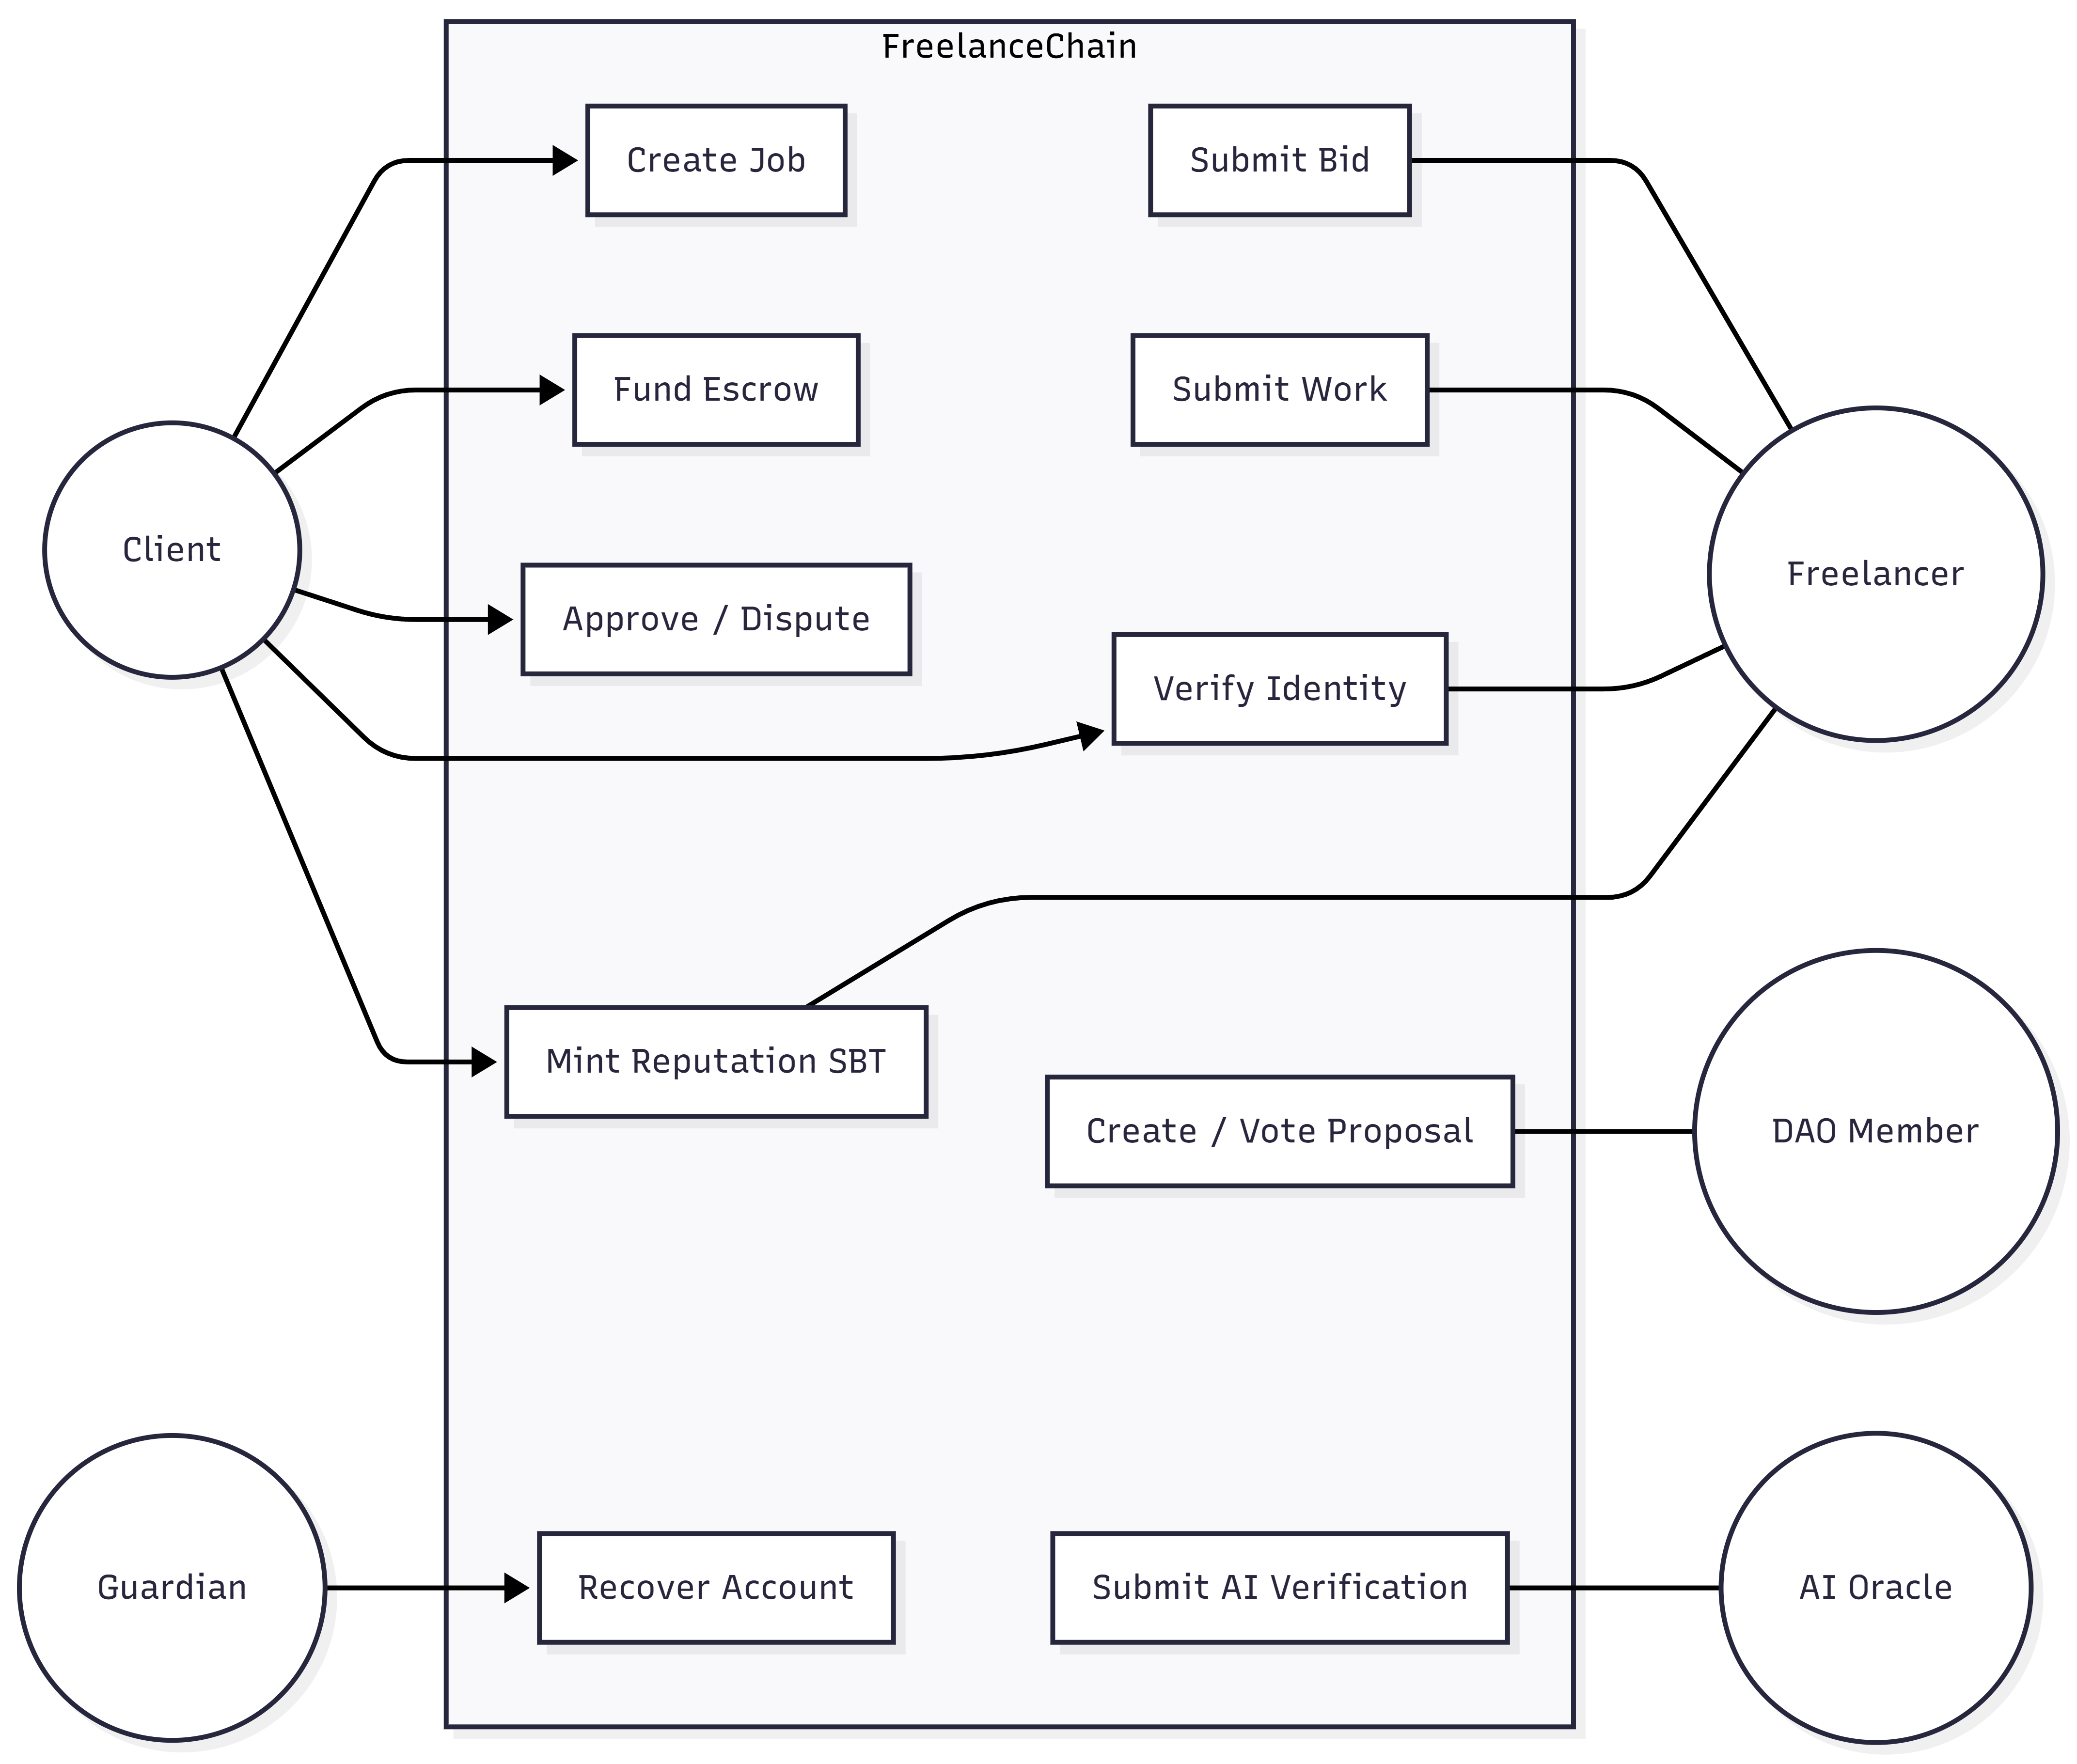
\includegraphics[width=0.8\textwidth]{usecase.png}
    \caption{General use case diagram of FreelanceChain.}
    \label{fig:general_usecase}
\end{figure}

\subsection{Business Process: Complete Engagement}
\label{subsection:2.2.4}

A complete freelance engagement proceeds as follows: (i)~the client invokes \emph{create\_job}; (ii)~freelancers invoke \emph{submit\_bid} with proposed budget, timeline, and optionally a CV URI; (iii)~the client (optionally aided by AI risk assessment) invokes \emph{select\_bid}; (iv)~the client funds escrow via \emph{deposit\_token\_escrow} or per-milestone \emph{fund\_milestone}; (v)~the freelancer submits deliverables; (vi)~the client either approves (\emph{release\_token\_escrow} or \emph{approve\_milestone}) or initiates a dispute (\emph{open\_token\_dispute}); and (vii)~each party may mint a reputation SBT via \emph{mint\_reputation\_sbt}. Figure~\ref{fig:business_process} renders this flow as a sequence.

\begin{figure}[H]
    \centering
    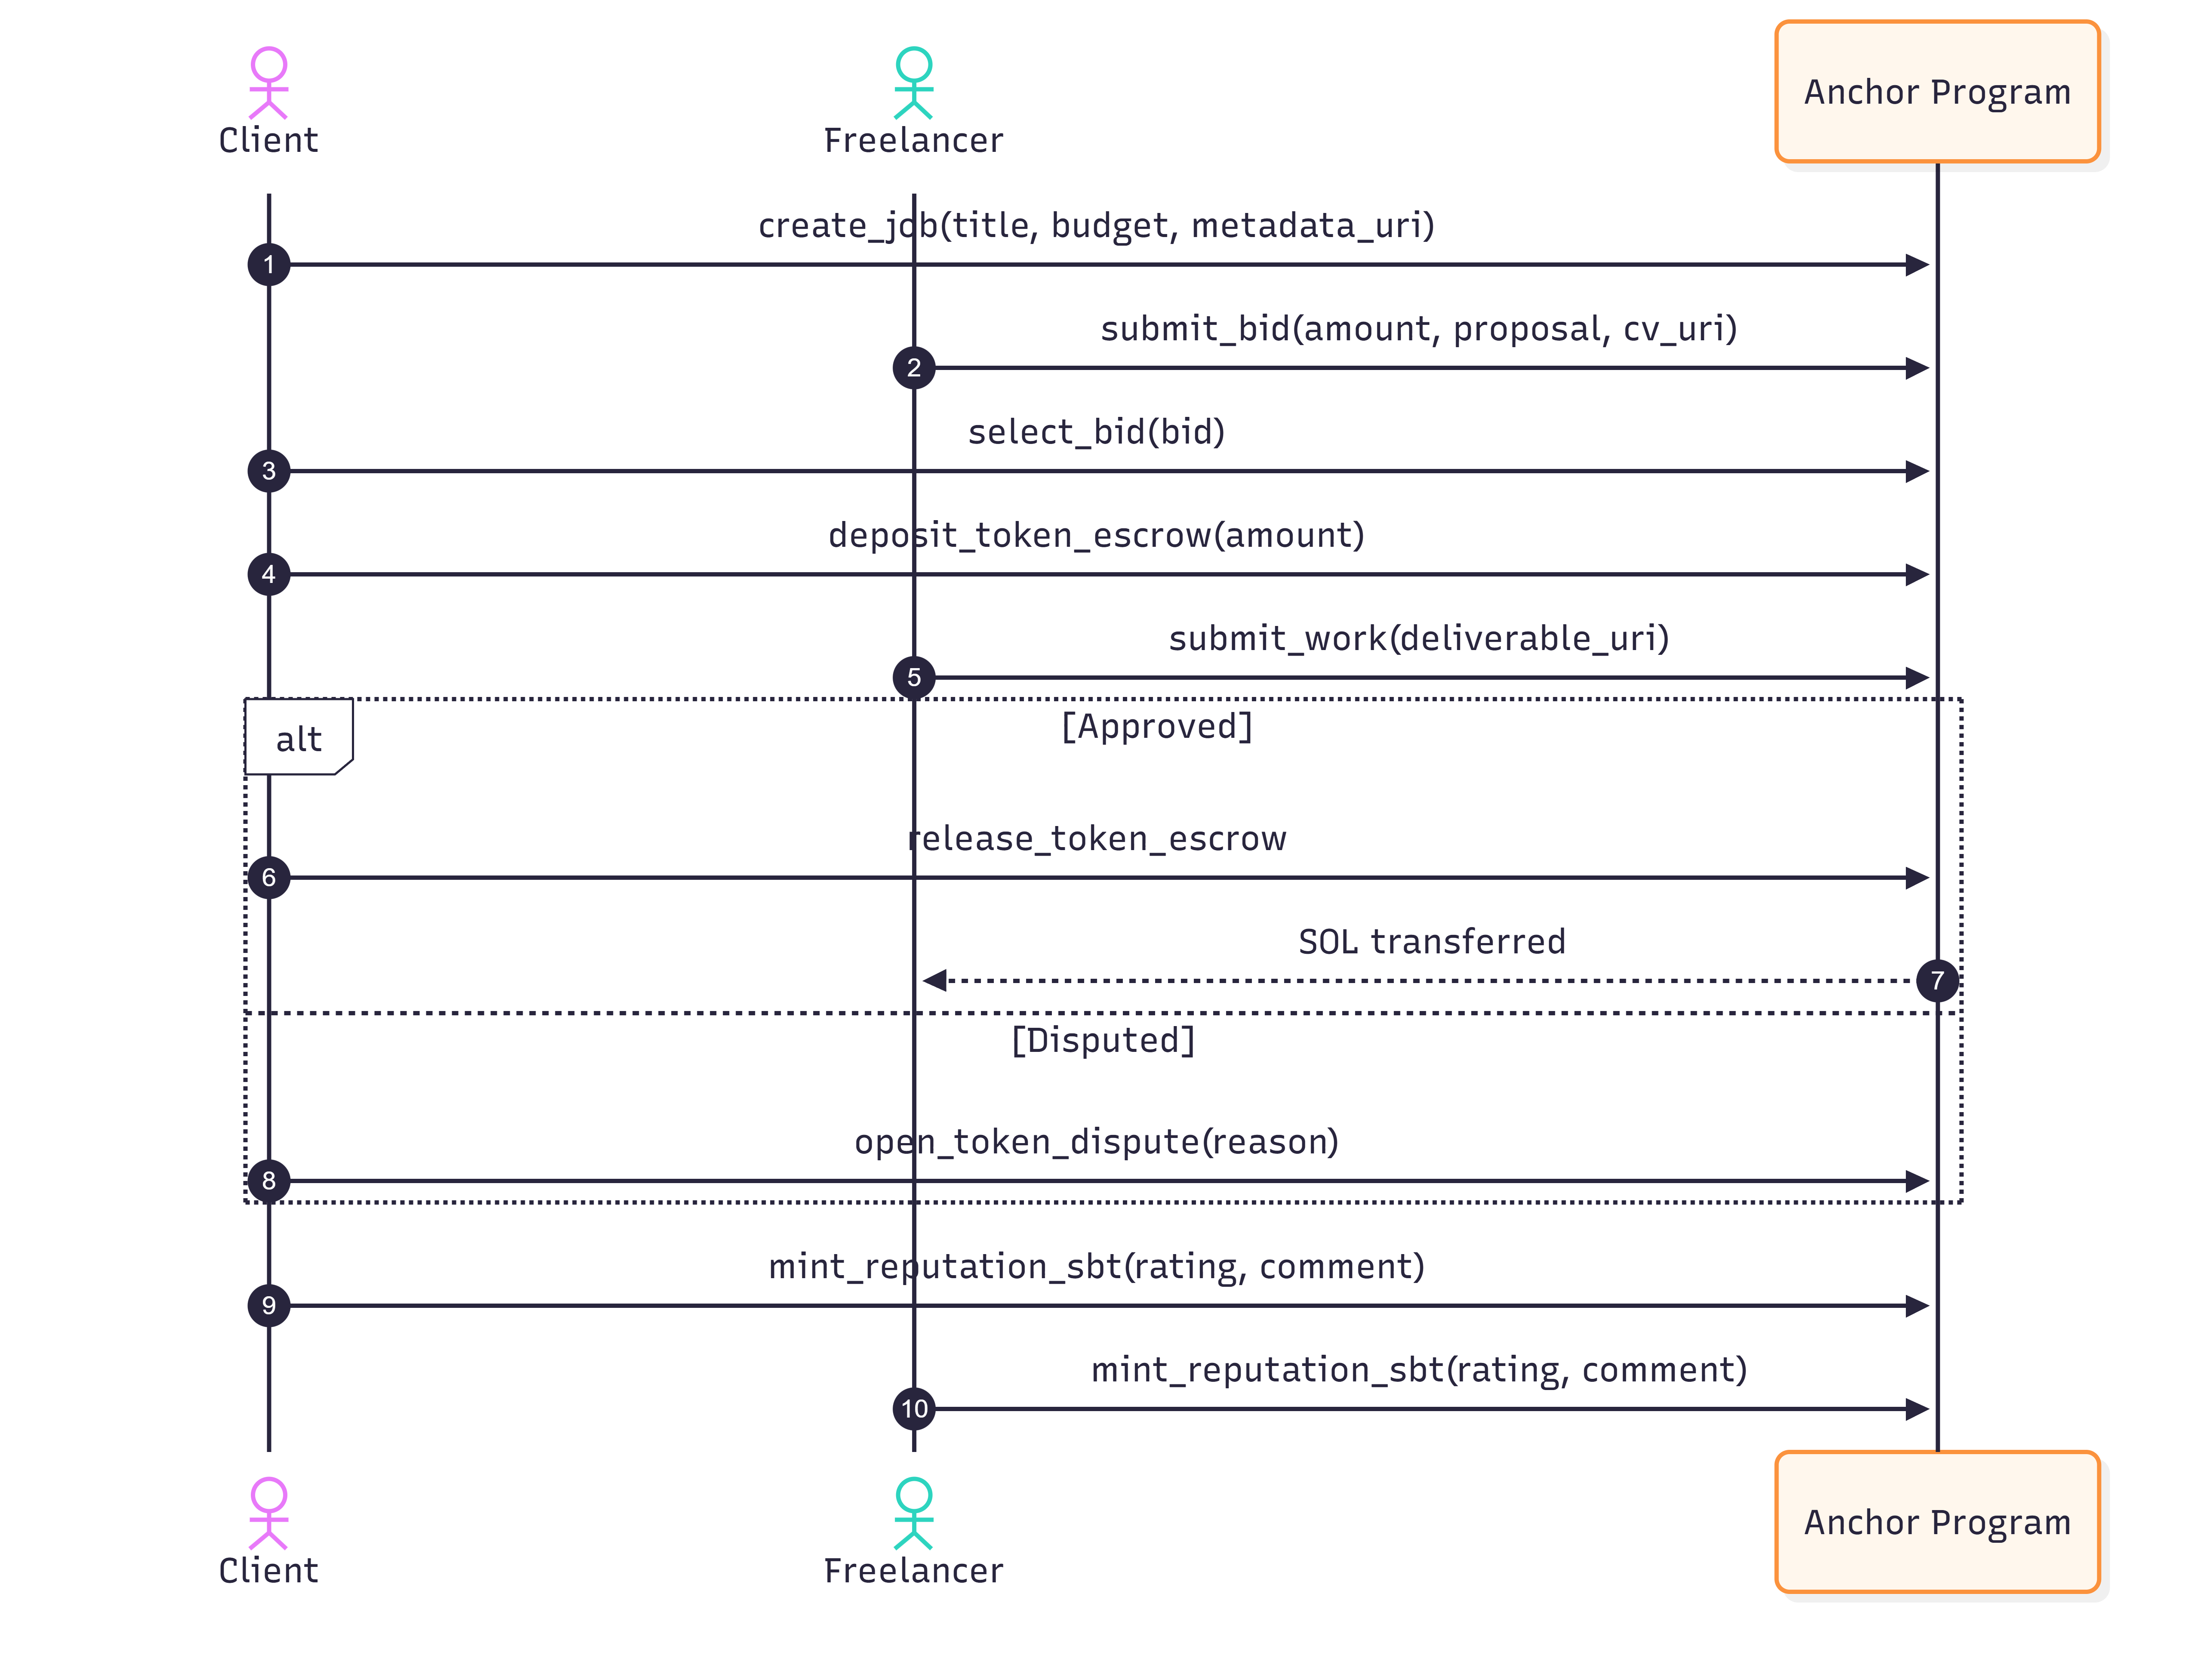
\includegraphics[width=1.0\textwidth]{sequence_diagram.png}
    \caption{Business process: complete freelance engagement.}
    \label{fig:business_process}
\end{figure}


\section{Critical Use Cases}
\label{section:2.3}

This section specifies four representative use cases; the remainder are deferred to Appendix~\ref{appendix:usecases}.

\begin{table}[H]
\centering
\caption{UC-01: Create and Fund Milestone Escrow.}
\label{table:uc01}
\small
\begin{tabular}{|l|p{9.5cm}|}
\hline
\textbf{Actor} & Client \\ \hline
\textbf{Preconditions} & Wallet connected; freelancer selected; job status \emph{InProgress}. \\ \hline
\textbf{Main flow} & Client defines 1--10 milestones (title, description, SOL amount); system validates aggregate amount $\leq$ job budget; \emph{init\_job\_milestones} is invoked; per-milestone \emph{fund\_milestone} calls lock SOL in each milestone PDA. \\ \hline
\textbf{Postconditions} & Milestone PDAs created; SOL locked in each milestone escrow. \\ \hline
\end{tabular}
\end{table}

\begin{table}[H]
\centering
\caption{UC-02: Submit Bid with CV.}
\label{table:uc02}
\small
\begin{tabular}{|l|p{9.5cm}|}
\hline
\textbf{Actor} & Freelancer \\ \hline
\textbf{Preconditions} & Wallet connected; job status \emph{Open}; no prior bid by the same freelancer. \\ \hline
\textbf{Main flow} & Freelancer enters proposed budget (SOL), proposal text, and timeline (days); optionally uploads a CV to \gls{ipfs} and embeds the resulting URI; signs and submits \emph{submit\_bid}. \\ \hline
\textbf{Postconditions} & Bid PDA initialized with status \emph{Pending} and surfaces in the client's bid list. \\ \hline
\end{tabular}
\end{table}

\begin{table}[H]
\centering
\caption{UC-03: KYC Identity Verification.}
\label{table:uc03}
\small
\begin{tabular}{|l|p{9.5cm}|}
\hline
\textbf{Actor} & Freelancer or Client \\ \hline
\textbf{Preconditions} & Wallet connected; functional webcam; government-issued identity document. \\ \hline
\textbf{Main flow} & User selects document type and uploads an ID photograph; \emph{face-api.js} extracts a descriptor $\mathbf{d}_{\text{doc}}$; user captures a webcam selfie yielding $\mathbf{d}_{\text{selfie}}$; system computes $\delta = \|\mathbf{d}_{\text{doc}} - \mathbf{d}_{\text{selfie}}\|_2$; if $\delta < 0.50$, \emph{finalize\_kyc} writes the result to chain. The current prototype performs only a single still-frame webcam capture and does not implement active liveness detection (e.g., blink or head-turn challenges); this is acknowledged as a limitation (Section~\ref{section:5.3}). \\ \hline
\textbf{Postconditions} & \emph{KycRecord} PDA initialized with \emph{Verified} or \emph{Rejected}; \emph{VerifiedBadge} surfaces on the profile. \\ \hline
\end{tabular}
\end{table}

\begin{table}[H]
\centering
\caption{UC-04: Open and Resolve Dispute.}
\label{table:uc04}
\small
\begin{tabular}{|l|p{9.5cm}|}
\hline
\textbf{Actor} & Either party (initiator); DAO arbitrators (resolvers) \\ \hline
\textbf{Preconditions} & Job status \emph{InProgress} or \emph{WaitingForReview}; escrow funded. \\ \hline
\textbf{Main flow} & Initiator invokes \emph{open\_token\_dispute} with rationale; escrow transitions to \emph{Disputed} and funds are frozen; arbitrators review evidence and vote; upon consensus, the contract transfers escrowed funds to the prevailing party. \\ \hline
\textbf{Postconditions} & Funds distributed; job status reflects the outcome. \\ \hline
\end{tabular}
\end{table}

Three further use cases -- \textit{Mint Reputation SBT}, \textit{Create/Vote on Governance Proposal}, and \textit{Social Recovery of Wallet Access} -- are specified analogously in Appendix~\ref{appendix:usecases}.

\section{Non-Functional Requirements}
\label{section:2.4}

\textbf{Performance.} On-chain instructions should confirm within one second on Devnet under nominal network conditions; the front-end should achieve a Time-to-Interactive below three seconds on a typical desktop; the browser-side face-recognition pipeline should complete within five seconds; a single Groq inference call should return within ten seconds.

\textbf{Security.} No party other than the contract logic should be able to access escrowed funds; the deployer key should not retain authority over user funds once initialization is complete. All on-chain instructions validate input ranges (rating $\in [1,5]$, fees $\in [1\%, 20\%]$, guardian count $\in [2,5]$). The KYC module rejects matches with $\delta \geq 0.50$ and prohibits duplicate identity-document submissions per wallet. No raw biometric data -- neither images nor 128-dimensional descriptors -- is transmitted to any external server. Within the scope of this prototype the program has not undergone third-party security audit; the threat model and known limitations are documented in Section~\ref{section:4.6}.

\textbf{Usability.} Job listings, freelancer profiles, and informational pages are accessible without a connected wallet; the system supports the Phantom wallet adapter; transaction failures are surfaced as human-readable messages.

\textbf{Technical.} Solana Devnet as the deployment network; Anchor~0.30.1; Next.js~14 with TypeScript and React~18; \gls{ipfs} for document storage and browser \emph{localStorage} for session-scoped caching; Chromium-based browsers with webcam access. The concrete Devnet program address is treated as a deployment artifact and reported with the implementation environment in Chapter~4 rather than as a requirement.

In summary, the surveyed platforms exhibit complementary deficiencies that motivate the unified architecture proposed in subsequent chapters. The requirements derived herein -- subject to the limitations of the informal survey described above -- drive the architectural decisions of Chapter~4 and Chapter~5.
